\documentclass{beamer}
\usepackage[utf8]{inputenc}
\usepackage[bahasai]{babel}
\usepackage{amsmath}
% to continu numbering
\newcounter{saveenumi}
\newcommand{\seti}{\setcounter{saveenumi}{\value{enumi}}}
\newcommand{\conti}{\setcounter{enumi}{\value{saveenumi}}}
\resetcounteronoverlays{saveenumi}

\title{Turunan Fungsi}
\author{bagustris}
\date{\today}
\begin{document}
	\frame{\titlepage}
	% \frame{
	% 	\frametitle{Table of Contents}
	% 	\tableofcontents
	% }
	
\begin{frame}[t,fragile]{Overview}
\tableofcontents
\end{frame}

\section{Limit Fungsi}
\begin{frame}[t, fragile] {Limit fungsi}
\underline{Definisi:} \\
Fungsi $y=f(x)$ dikatakan mempunyai Limit L untuk $x$ mendekati $a$ ditulis  $$\lim_{x\to a} f(x) = L$$ 
Jika untuk setiap bilangan $\varepsilon > 0$ (yang bagaimanapun kecilnya) dapat ditunjuk bilangan $\delta > 0$ (biasanya bergantung pada $\varepsilon$) sedemikian hingga $| f(x) = L | < \varepsilon$ untuk $ 0 < |x -a| < \delta$.\\
\vskip5pt
Dalil-dalil limit: \\
Jika $\lim_{x\to a} f(x) = L$ dan $\lim_{x\to a} g(x) = M$ maka : \\
\begin{enumerate}
\item $\lim_{x\to a} {f(x) \pm g(x) }= L \pm M$
\item $\lim_{x\to a} {f(x) . g(x) }= L . M$
\item $\lim_{x\to a} \dfrac{1}{f(x)}= \dfrac{1}{L}, ~~jika~ L \neq 0 $
\item $\lim_{x\to a} \dfrac{f(x)}{g(x)}= \dfrac{L}{M}, ~~jika~ M \neq 0 $
\end{enumerate}
\end{frame}

\begin{frame}[t, fragile] {Fungsi Kontinyu}
\underline{Definisi:} Suatu fungsi $y=f(x)$ dikatakan kontinyu di $x=a$ jika 
\begin{enumerate}
\item f(a) ada
\item $\lim_{x\to a} f(a)= ada$
\item $\lim_{x\to a} f(x) = f(a)$
\end{enumerate}
Tegasnya $f(x)$ disebut kontinyu di $x=a$ jika $$\lim_{x\to a} f(x) = f(a)$$ ada. \\
\vskip5pt
Jika $f(x)$ kontinyu pada setiap titik dari suatu interval maka $f(x)$ dikatakan kontinyu pada interval itu. \\
\vskip5pt
Jika satu alasan atau lebih dari syarat-syarat kontinyuitas diatas tidak terpenuhi, maka $f(x)$ dikatakan diskontinyu di $x=a$.

\end{frame}

%\section{Turunan}
%\begin{frame}[t, fragile]{Turunan fungsi}
%\includegraphics[width=3.5in]{pict/turunan.png}
%\end{frame}

\section{Turunan}
\begin{frame}[t, fragile]{Turunan fungsi}
\begin{itemize}
\item Limit fungsi ketika $x$ mendekati nilai a didefinisikan sbg,
$$
\lim_{x\rightarrow a}f(x)=L 
$$
\item Kalkulus diferensial $\rightarrow$ laju perubahan fungsi $\Delta f$ terhadap perubahan waktu $\Delta x$.
\item Laju perubahan $\rightarrow$ rasio dari perubahan fungsi $\Delta f$ terhadap perubahan waktu $\Delta x$. 
\item Sepanjang interval $\Delta x$, fungsi berubah dari $f(x)$ menjadi $f(x+\Delta x)$, sehingga
$$ \Delta f = f(x+\Delta x) - f(x) $$
\item Apabila kita memperkecil $\Delta x$ maka turunan $\Delta f$ / $\Delta x$ sama dengan mencari limitnya, 
$$\frac{df}{dx}=\lim_{\Delta x \rightarrow 0} \frac{\Delta f}{\Delta x}=\lim_{\Delta x \rightarrow 0} \frac{f(x + \Delta x)-f(x)}{\Delta x}.$$
\end{itemize}
\end{frame}

\begin{frame}[t, fragile]{Turunan fungsi}
\begin{center}
\includegraphics[width=3in]{pict/turunan}
\end{center}
\end{frame}

\begin{frame}[t, fragile]{Soal}
Dengan menggunakan definisi turunan  $\Bigl( \dfrac{df}{dx}=\lim_{x\to 0}\dfrac{\Delta{f}}{\Delta{x}}=\dfrac{f(x+h)-f(x)}{h}\Bigr)$, dapatkan turunan dari fungsi berikut:
\begin{enumerate}
\item $f(x) = x^2$
\item $f(x) = x^3$
\item $f(x) = 2x$
\item $f(x) = \sin (x)$
\end{enumerate}
\end{frame}

\section{Logaritma Natural}
\begin{frame}[t, fragile]{Logaritma dan Bilangan Natural}
\begin{center}
\fbox{$^a\log{b} = c$} $\Longrightarrow$ logaritma Brigg 
\end{center}
Syarat: $a > 0, a \neq 1, b > 0, c = $semua bil. real \\
\hspace{33px} $a$ disebut bilangan pokok bilangan logaritma \\
Sifat:
$$^a\log{b}=\dfrac{\log{b}}{\log{a}}=\dfrac{^2\log{b}}{^2\log{a}}=\dfrac{^n\log{a}}{^n\log{b}}$$
Bilangan natural/alam= e = 2.71828183 \\
$$^a\log{b}=\dfrac{\log{b}}{\log{a}}=\dfrac{^e\log{b}}{^e\log{a}}=\dfrac{^e\ln{a}}{^e\ln{b}}$$
$$^e \log {x} = \ln {x}$$
\begin{center}\fbox{$y=\ln[f(x)] \rightarrow y'=\dfrac{f'(x)}{f(x)}$}
\end{center}
\end{frame}

\begin{frame}[t, fragile]{Sifat-sifat Turunan}
Jika $u = f(x), v= g(x)$, maka: \\
\begin{enumerate}
\item $y = u \pm v \Longrightarrow y'= u' \pm v'$
\item $y = uv \Longrightarrow y'=u'v + uv'$
\item $y = \dfrac{u}{v} \Longrightarrow y'=\dfrac{u'v-uv'}{v^2}$
\item $y=u^v \Longrightarrow y'=u^v\bigl(v' \ln u+v \dfrac{u'}{u}\bigr)$
\end{enumerate}
Beberapa rumus turunan[1]:
\begin{enumerate}
\item $y=C \Longrightarrow y'=0$
\item $ y = x^n \Longrightarrow y'=nx^{n-1}$
\item $y=e^x \Longrightarrow y'=e^x$
\item $y=\ln x \Longrightarrow y'=\dfrac{1}{x}$
\item $y= ^a\log x \Longrightarrow y'= \dfrac{1}{x \ln a}$
\item $y= a^x; (a>0, a \neq 1) \Longrightarrow y'=a^x \ln a $
\seti
\end{enumerate}
\end{frame}

\begin{frame}[t, fragile]{Beberapa Rumus Turunan[2]}
\begin{enumerate}
\conti
\item $y=\sin{x} \Longrightarrow y'=\cos x$
\item $y=\cos x \Longrightarrow y'= - \sin x$
\item $y= \tan x \Longrightarrow y'=\sec^2 x$
\item $y= \cot x \Longrightarrow y' = -\csc ^2 x$
\item $y= \sec x \Longrightarrow y' = \sec x \tan x$
\item $y= \csc x \Longrightarrow y'= - \csc x \cot x$
\item $y= \ln |\sin x| \Longrightarrow y'= \cot x$
\item $y= \ln |\cos x| \Longrightarrow y'= - \tan x$
\item $y= \ln |\sec x + \tan x| \Longrightarrow y'= \sec x$
\item $y= \ln |\csc x - \cot x| \Longrightarrow y'= \csc x$
\item $y= \ln | x + \sqrt{x^2 \pm a} | \Longrightarrow y'= \dfrac{1}{\sqrt{x^2\pm a}}$
\seti
\end{enumerate}
\end{frame}

\begin{frame}[t, fragile]{Beberapa Rumus Turunan[3]}
\begin{enumerate}
\conti
\item $y= \arcsin x \Longrightarrow y'= \dfrac{1}{\sqrt{1-x^2}}$
\item $y= \arccos x \Longrightarrow y'= \dfrac{-1}{\sqrt{1-x^2}}$
\item $y= \arctan x \Longrightarrow y'= \dfrac{1}{1+x^2}$
\item $y= arccot ~x \Longrightarrow y'= \dfrac{-1}{1+x^2}$
\item $y= arcsec ~x \Longrightarrow y'= \dfrac{1}{x \sqrt{x^2-1}}$
\item $y= arccsc ~x \Longrightarrow y'= \dfrac{-1}{x \sqrt{x^2-1}}$
\end{enumerate}
\end{frame}

\section{Fungsi Hiperbolik}
\begin{frame}[t, fragile]{Fungsi Hiperbolik}
Definisi:\\
$$\sinh x=\dfrac{1}{2}(e^x - e^ {-x})$$\\
$$\cosh x=\dfrac{1}{2}(e^x + e^ {-x})$$\\
Sifat-sifat:\\
\begin{enumerate}
\item $\cosh^2 x - \sinh^2 x=1$
\item $\sinh (x \pm y) = \sinh x \cosh y \pm \cosh x \sinh y$
\item $\cosh (x \pm y) = \cosh x \cosh y \pm \sinh x \sinh y$
\end{enumerate}
Turunan:\\
\begin{enumerate}
\item $y=\sinh x \Longrightarrow y'=\cosh x$
\item $y=\cosh x \Longrightarrow y'=\sinh x$
\item $y=\tanh x \Longrightarrow y'=sech ^2 x$
\end{enumerate}
\end{frame}

\section{Aturan Berantai}
\begin{frame}[t, fragile]{Aturan berantai}
Jika $y=f(u)$ dan $u=g(x)$ maka:\\
$$\dfrac{dy}{dx}=\dfrac{dy}{du}.\dfrac{du}{dx}$$
Jika $y=f(u)$, $u=g(v)$ dan $v=h(x)$ maka:\\
$$\dfrac{dy}{dx}=\dfrac{dy}{du}.\dfrac{du}{dv}.\dfrac{dv}{dx}$$
\underline{Soal:}\\
\begin{enumerate}
\item $y=(2x+5)^5 \Longrightarrow~ y'=...?$
\item $y=(x^2+2)^4 \Longrightarrow~ y'=...?$
\end{enumerate}
\end{frame}

\section{Turunan Tingkat Tinggi}
\begin{frame}[t, fragile]{Turunan tingkat tinggi}
$y=f(x) \Longrightarrow$ turunan ke 1 terhadap x adalah $ y'=f'(x)$\\
\hspace*{62px} turunan ke 2 terhadap x adalah $ y''=y^{(2)}=f^{(2)}(x)$\\
\hspace*{62px} turunan ke 3 terhadap x adalah $ y'''=y^{(3)}=f^{(3}(x)$\\
\hspace*{62px} ...dst \\
\hspace*{62px} turunan ke n terhadap x adalah $y^{(n)}=f^{(n)}(x)$\\
\underline{Soal:}\\
\begin{enumerate}
\item $y=e^{ax} \rightarrow y^{(n)}=....? $
\item $y=\sin x\rightarrow y^{(n)}=....? $
\end{enumerate}
\end{frame}

\section{Rumus Leibnitz}
\begin{frame}[t, fragile]{Rumus Leibnitz}
$D=\dfrac{d}{dx}$ operator turunan; $D^2=\dfrac{d^2}{dx^2}$;\\
$$D=\dfrac{d}{dx} \rightarrow ~operator~turunan~tingkat~n$$
Jika $y=UV$ dimana $U=f(x)$ dan $V=g(x)$ maka turunan $n$ dari $y$ terhadap $x$ dinyatakan dengan $y^({n)}=D^n(UV)$ dan dirumuskan sbb:
\begin{multline}
y^n(UV)=UD^nV+nDUD^{n-1}V+\dfrac{1}{2!}n(n-1)D^2UD^{n-2}V+\\
\dfrac{1}{3!}n(n-1)D^3UD^{n-3}V+...
\end{multline}
Bukti:\\
$y=UV \Longrightarrow y'=UV'+U'V$ \\
\hspace{60px}$y"=UV"+2U'V'+U"V$\\
\hspace{60px}$y^{(3)}=UV^{(3)}+3U'V^{(2)}+3U^{(2)V'}+U^{(3)}V$
\end{frame}

\section{Turunan fungsi parametrik}
\begin{frame}[t, fragile]{Turunan fungsi parametrik}
Jika $x=f(t)$ dan $y=g(t)$ maka, \\
\begin{center}
\fbox{$y'=\dfrac{\dfrac{dy}{dt}}{\dfrac{dx}{dt}}; y"=\dfrac{\dfrac{dy'}{dt}}{\dfrac{dx}{dt}}; ...$}
\end{center}
$$y^{(n)}=\dfrac{\dfrac{dy^{(n-1)}}{dt}}{\dfrac{dx}{dt}}$$
\underline{Soal:}\\
Dapatkan $y"$ dari $x = a \cos t$ dan $y= b \sin t$
\end{frame}

\section{Menurunkan Fungsi Implisit}
\begin{frame}[t, fragile]{Menurunkan fungsi implisit}
$y'$ dari $f(x,y) = 0$ didapat sebagai berikut:
\begin{enumerate}
\item Jika mungkin $y$ dinyatakan sebagai fungsi explisit dalam x \\
      Contoh: $x^2+y-3=0 \Longrightarrow y=3-x^2$\\
        \hspace{132px}$y'=-2x$
\item Setiap suku dalam $f(x,y)=0$ diturunkan terhadap x. Karena $y$ fungsi $x$ maka setiap kali menurunkan $y$ harus digandakan dengan $y'$, kemudian hubungan yang didapat diselesaikan ke $y'$.\\
      Contoh:\\
      $x^3+y^3-3axy=0 $\\
      $3x^2+3y^2y^1-3a(y+xy')=0$\\
      $3(ax-y^2)y^1=3(x^2-ay) \Longrightarrow y'=\dfrac{x^2-ay}{ax-ay}$
\end{enumerate}
\end{frame}

\begin{frame}[t, fragile]{Soal}
Dapatkan $y'$ dari:
\begin{itemize}
\item $y=x \sinh{x}$
\item $y=\ln\sqrt{2x+1}$
\item $y=e^{2x+y} + \sin({x+2y})$
\item $y=\ln{\dfrac{x+1}{x-1}}$
\end{itemize}
\end{frame}
\end{document}
